\subsection{Learning Setup}
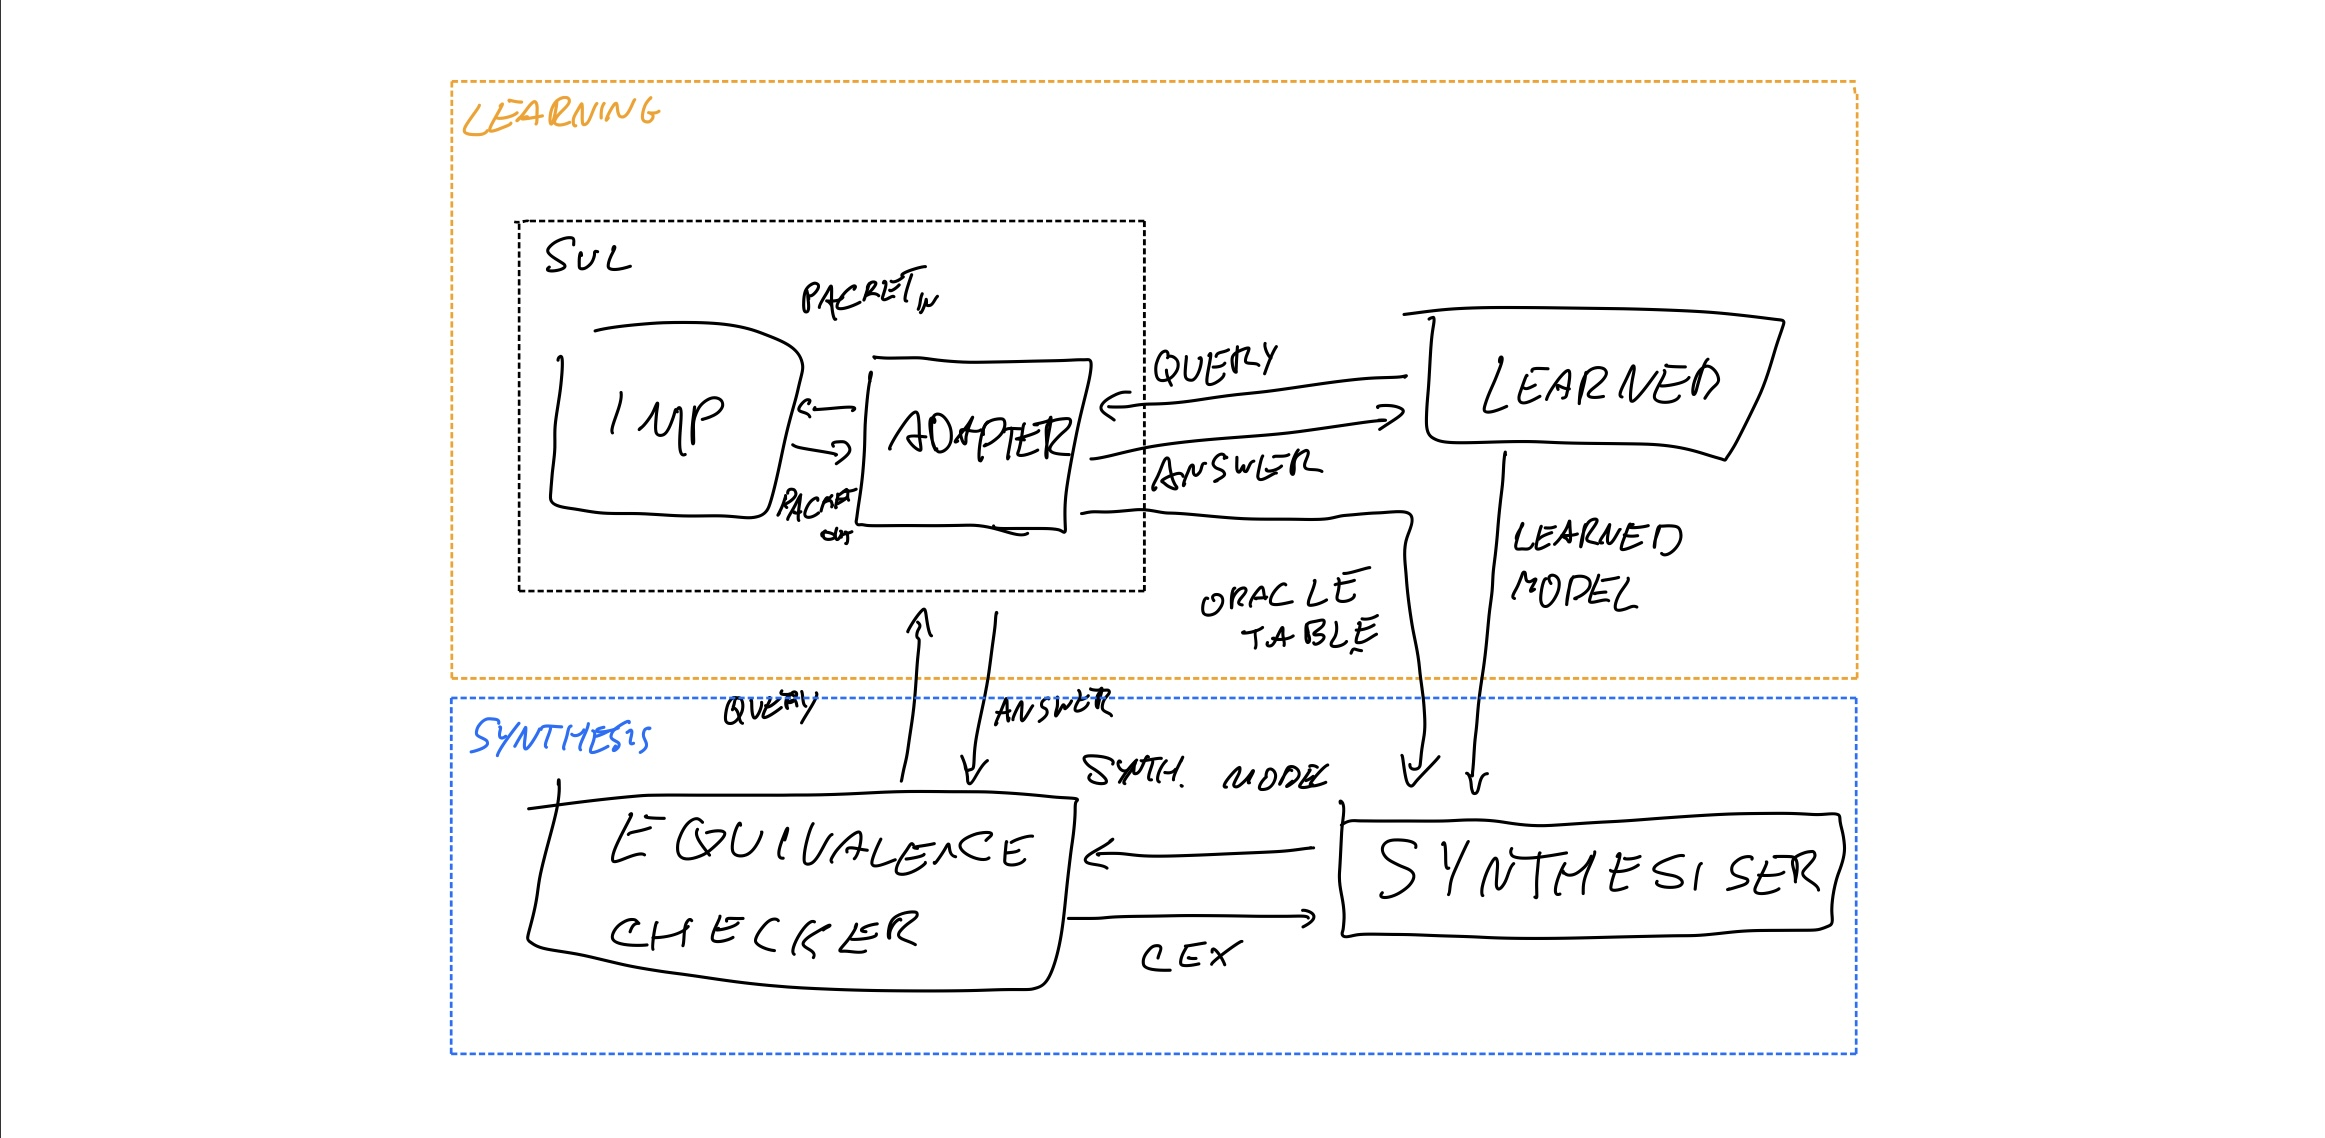
\includegraphics[width=\textwidth]{graphics/setup-drawing.jpg}


\tikzstyle{module} = [rectangle, draw,
    text width=5em, text centered, rounded corners, 
    minimum height=4em, node distance=5cm]

\tikzstyle{closemodule} = [rectangle, draw,
    text width=5em, text centered, rounded corners, 
    minimum height=4em, node distance=2cm]

\tikzstyle{line} = [draw, -latex']


\begin{figure}
    \centering
    \begin{tikzpicture}[node distance = 2cm, auto]
        % Place nodes
        \node [module] (sul) {System under learning};
        \node [module, right of=sul] (l*) {Learn Lib};
        \node [module, right of=l*] (synth) {Synthesizer};
        \node [closemodule, below of=l*] (tester) {Tester};
        
        \path [line] (sul) edge [bend left = 20] node {$a$-membership queries}(l*);
        \path [line] (sul) edge [bend right = 20] node {$a$-equivalence queries}(l*);
        \path [line] (l*) -- node {get $a$-machine}(synth);
        \path [line] (synth) edge [bend right = 20] node {get $w$-machine}(tester);
        \path [line] (tester) edge [bend right = 40] node {get c. example}(synth);
        \path [line] (sul) edge [bend right = 40] node {$w$-membership}(tester);
        
    \end{tikzpicture}
    \caption{
    It ugly.
    }
\end{figure}
Our algorithm starts by learning a mealy machine over the abstractions $\hat\Sigma$ of the input alphabet $\Sigma$ and $\hat\Gamma$ of the output alphabet $\Gamma$.
\subsubsection{Implementation}
The implementation is the original SUL we are attempting to learn. It can only communicate using the concrete alphabets $\Sigma$ and $\Gamma$, and so in our setup it interacts only with the adapter. This module can be conveniently swapped with any other implementation of the same protocol.
\subsubsection{Adapter}

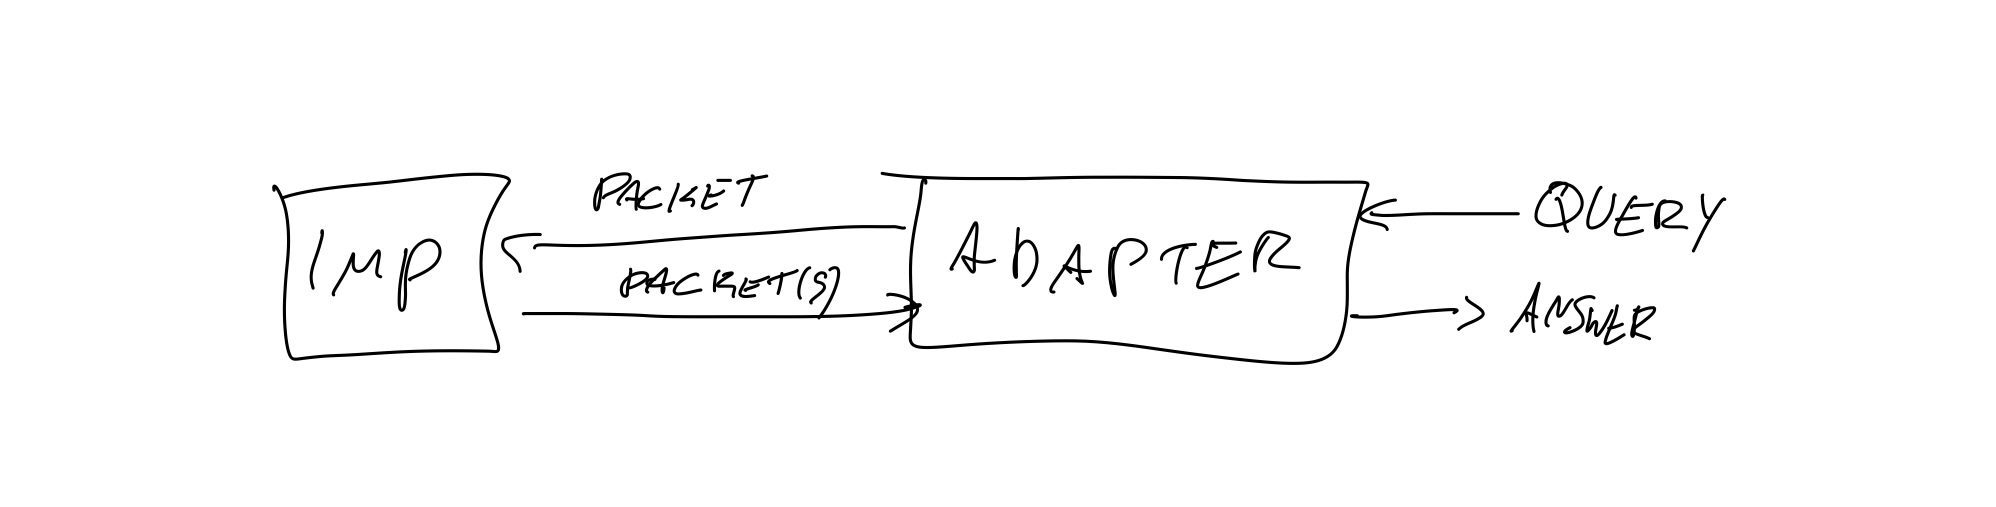
\includegraphics[width=\textwidth]{graphics/adapter-drawing.jpg}
A key part of interactive learning, is that the learner knows how to interact with the \sul. In some cases however, the \sul might use a very complex alphabet for communication, like specific packet formats and encrypted messages. 

We call the full detail represented in these symbols the concrete alphabets $\Sigma$ and $\Gamma$, for input and output symbols respectively. So even though a packet for example, is communicated as a sequence of binary digits $\mathbbm{2}^*$, the information those bits represent can be interpreted as a \textit{JSON} object containing the information of each field. 

In previous setups~\cite{tcp-learner} this component is called the \adapter, as it merely adapts the same data from a format to another, specifically, from sequences of concrete symbols to binary sequences. As such, it can be seen as a map of type $(\Sigma^* \times \Gamma^*) \to (\mathbbm{2}^* \times \mathbbm{2}^*)$.

We could then learn a state machine over these alphabets $\Sigma$ and $\Gamma$, knowing that they have a one-to-one native representation. However, often this is still not enough, as these concrete alphabets $\Sigma$ and $\Gamma$ might be too big for effective learning, or even infinite. As an example consider the concrete alphabets of a network packet format. These packets might have a \texttt{Packet Number} field, that is increasing and unique for each packet. We would then need to have an alphabet symbol for each of these packets, and even if that weren't an issue, this then combined with all the other possibilities for other counters gives us an extremely big alphabet. 

As such, it is common to learn instead over \textit{Abstract Alphabets} $\hat\Sigma$ and $\hat\Gamma$. These alphabets allow us to focus on the crucial aspects of the symbols by abstracting away details that would make the alphabet otherwise too big or infinite. This mapping however, is more complex than the \adapter, as the abstraction is a lossy conversion. When we abstract a concrete symbol to an abstract one, we are removing details we deem unnecessary for learning. However, these details are essential for the \adapter to communicate with the \sul, so we would need to determine this missing detailed information.

In the past~\cite{tcp-mapper}, this has been done with an extra element, the \mapper. The \mapper is an implementation of the Protocol logic that is able to abstract details away from a concrete alphabet to an abstract alphabet, and via the inverse construct these details, by running through the same logic that a normal implementation would. As an example, the \mapper in ~\cite{tcp-mapper} takes in a concrete TCP Packet TCP\{flags: \texttt{SYN}, Seq: \texttt{123}, Ack: \texttt{0}\} and produces an abstract TCP Packet TCP\{flags: \texttt{SYN}, Seq: $\top$, Ack: $\top$\} if it finds that the now abstract fields had valid concrete values. 

In the inverse, it has to be able to produce values that are valid, or invalid, as requested. As such, the \mapper can be seen as a function of type $(\hat\Sigma^* \times \hat\Gamma^*) \to (\Sigma^* \times \Gamma^*)$.

We found that this is a luxury that one cannot always afford. If the protocol relied on a logic of high complexity, including aspects like key derivation, encryption, or really symbols that contain a large number of fields to be abstracted, then this would mean programming an implementation logic of our own, that we trust to be correct and able to communicate with the \sul. 

There is a common expression in the field of Cryptography: \textit{Never roll your own Crypto.} This is because cryptographic algorithms tend to be of great complexity and have big consequences when they're incorrectly implemented. Thus it is preferred to use an existing implementation that has been widely used and so is more likely to be correct. We believe the same applies for the \mapper and \adapter in our case. 

As such, instead of having both a \mapper and then an \adapter, with a total of 2 maps being done of type $(\hat\Sigma^* \times \hat\Gamma^*) \to (\Sigma^* \times \Gamma^*) \to (\mathbbm{2}^* \times \mathbbm{2}^*)$, we instead have a single component, our \adapter, that is able to do a direct map of type $(\hat\Sigma^* \times \hat\Gamma^*) \to (\mathbbm{2}^* \times \mathbbm{2}^*)$, by combining the functionality of the two components used in ~\cite{tcp-learner}, while being able to keep a record of the intermediate values $(\Sigma^* \times \Gamma^*)$ used in the conversion. We call this the \at.

Furthermore, instead of coding all this logic ourselves, we adapted a common implementation that was specifically built for testing and is widely used by the implementers, and rely on it to both do the abstraction logic, and native formatting, as a normal implementation would. 

Now that we have constructed an abstraction that produces a finite alphabet, and we have effective ways of querying over this alphabet, we can learn this state machine using existing learning algorithms.

\subsubsection{Learner}
With our abstractions we are now learning a classic state machine, and so can use any of the classic algorithms available to us.

\subsubsection{Synthesizer}
Once we have learned a the abstract state machine we will enrich the edges with information to learn the more complex inputs and outputs. We do this by taking the learned machine and the examples gathered in oracle table by the abstract learner, 
and synthesizing a $w$-machine that correctly produces the input and output examples.

\subsubsection{Equivalence Checker}
Once we have synthesized a $w$-machine we then generate input examples from our machine, 
pass this input into the system under learning,
and determine if the combined input and output are accepted.

\subsection{Minimal Example}
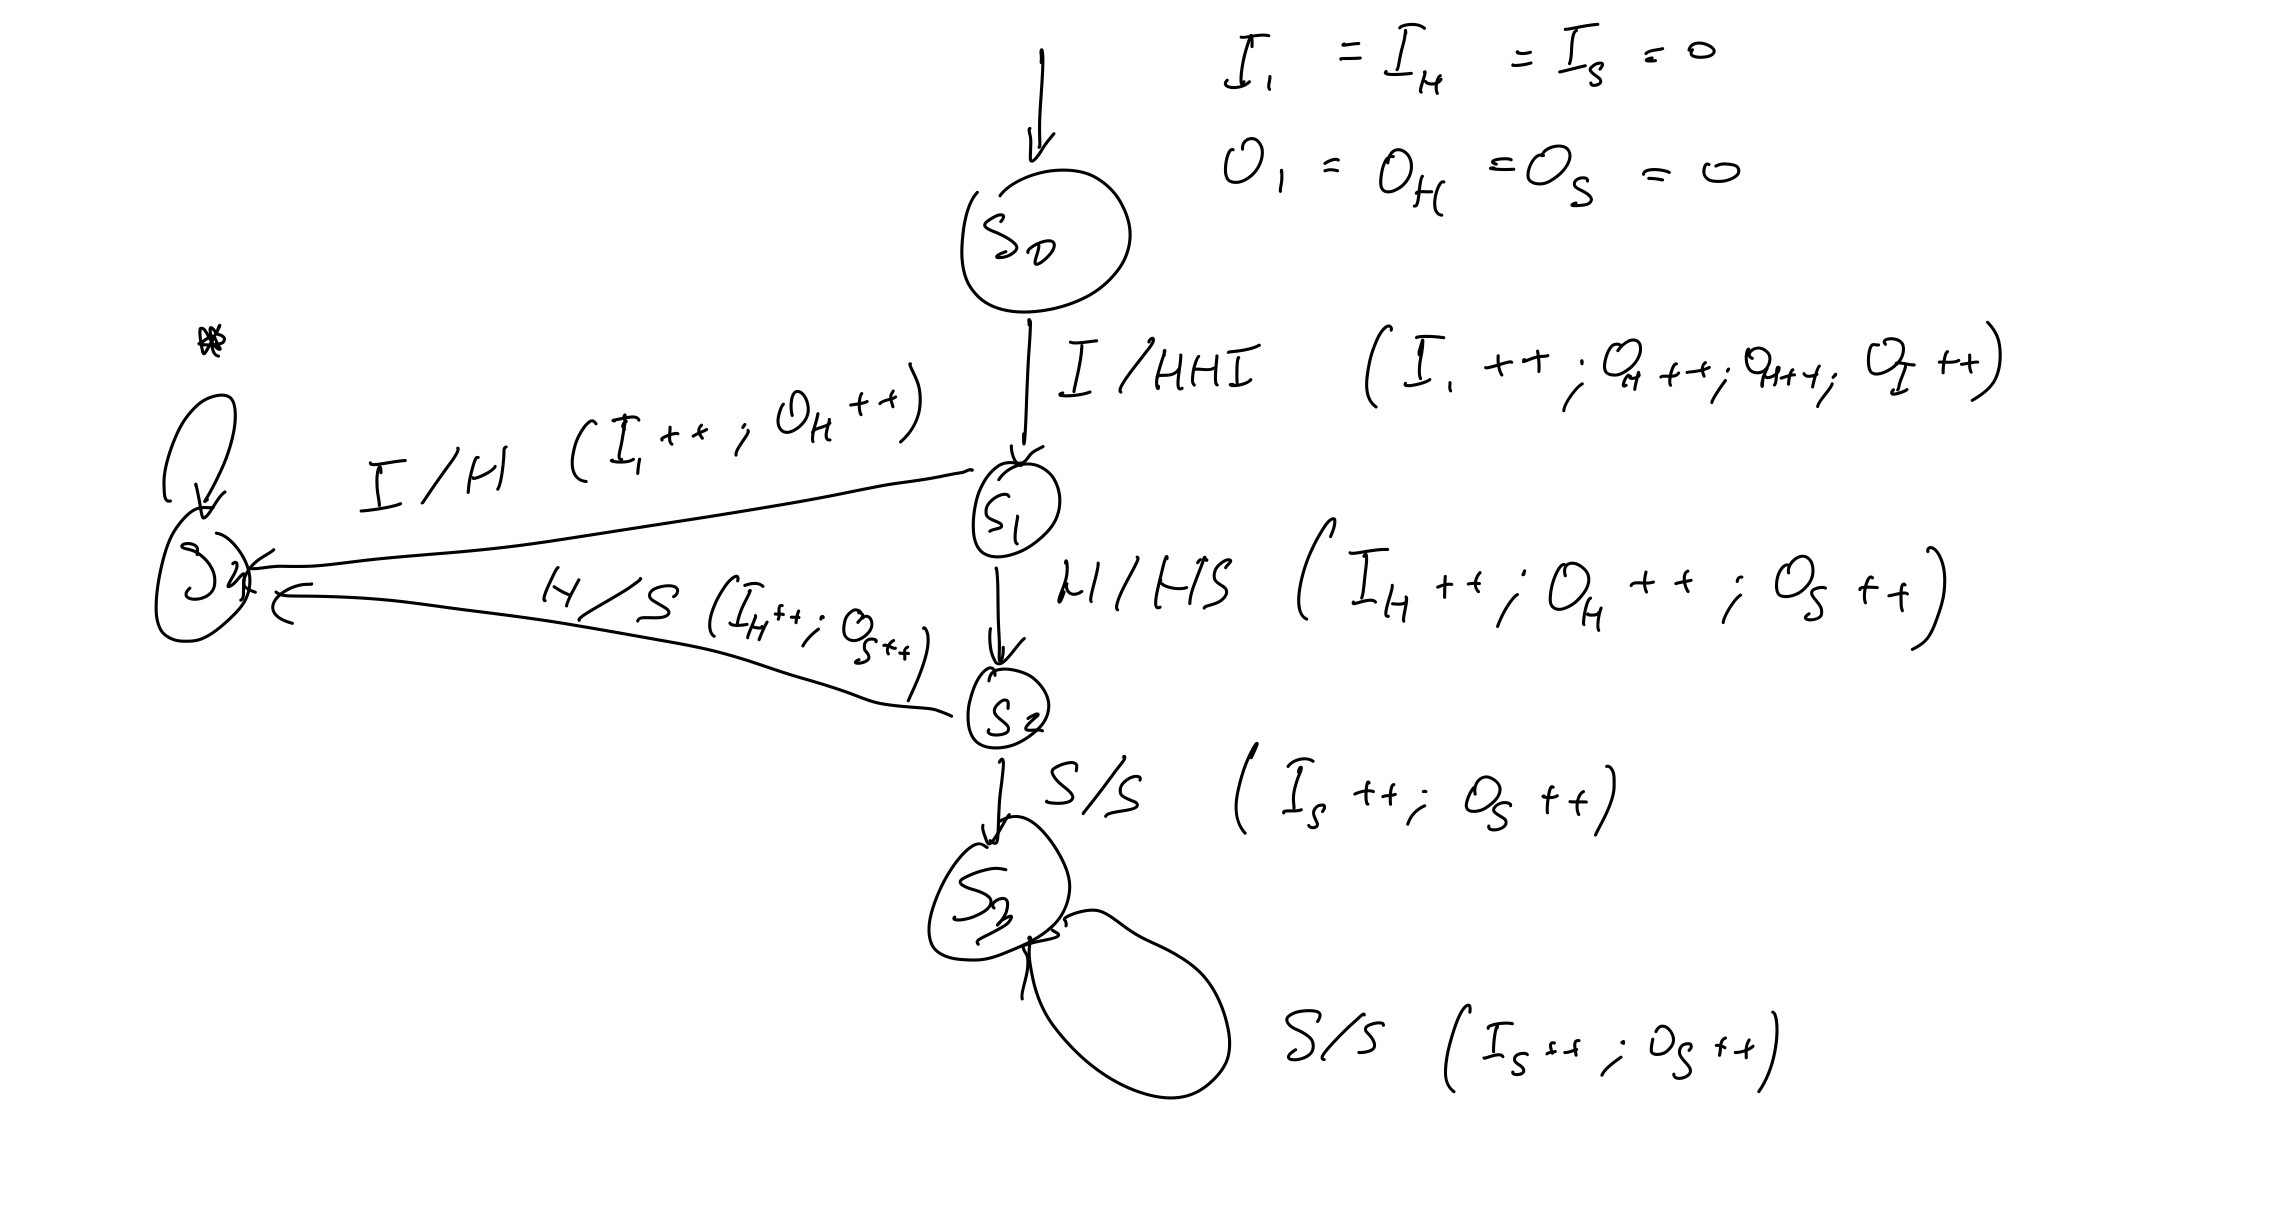
\includegraphics[width=\textwidth]{graphics/example-drawing.jpg}

%Informal problem def. - Explain the need for abstraction when learning, show how this removes information, demonstrate how this can sometimes be recovered with synthesis.  

%example + corresponding automaton. - simple example of the Big Counter Automaton, preferably abstract enough that it doesnt require background knowledge of the language.

%Eventually needs to have a run through of the algo – demonstrate automaton changing as the algorithm runs. 

\subsection{The Big Idea}